\section{Statistical analysis}
%
%%%%%%%%%%%%%%%%%%%%%%%%%%%%%%%%%%%%%%%%%%%%%%%%%%%%%%%%%%%
\subsection{Data} \label{s_sect:data}
%
%%%%%%%%%%%%%%%%%%%%%%%%%%%%%%%%%%%%
\subsubsection{Outcomes} \label{ss_sect:outcome}
%
On the one hand, the outcome for the \textbf{judgment task} was obtained following the procedure outlined in sections \ref{ss_sect:proc} and \ref{ss_sect:expset}, with the total number of judgments per procedure detailed in Table \ref{tab:allocation}.

On the other hand, the outcome from the \textbf{transcription task} was obtained following a two step procedure \citep{Boonen_et_al_2021}. First, we aligned the participant's orthographic transcriptions, at the utterance level, in a column-like grid structure similar to the one presented in Table \ref{tab:align_example}. This step was repeated for every one of the $6400$ transcriptions\footnote{\label{foot:doe}under DoE literature, the design corresponds to $32$ experimental units with $10$ replicates each, making a total of $320$ experimental runs. Moreover, we register $20$ duplicates (transcriptions) for each run, making a total of $6400$ transcriptions.} (see Section \ref{s_sect:JandT}). Lastly, we computed the entropy measure of the aligned transcriptions as in \citet{Shannon_1948}: 
%
\begin{equation} \label{eq:entropy}
	H = H(\pmb{p}) = \frac{-\sum_{i=1}^{n} p_{i} \cdot \log_{2}(p_{i})}{\log_{2}(N)}
\end{equation}
%
where $H$ is bounded in the continuum $[0,1]$, $n$ denotes the number of word occurrences, $p_{i}$ the probability of the word occurrence, and $N$ the total number of aligned transcriptions per utterance.
%
\begin{table}[h!]
	\centering
	\begin{tabular}{| c | ccccc | } 
		\hline
		Transcription & \multicolumn{5}{c |}{Utterance} \\ [0.5ex]
		\cline{2-6}
		number & 1 & 2 & 3 & 4 & 5 \\ [0.5ex] 
		\hline\hline
		1 & de & jongen & ziet & een & kikker \\ 
		  & the & boy & see & a & frog \\ 
		\hline
		2 & de & jongen & ziet & de & [X] \\
		  & the & boy & sees & the & [X] \\ 
		\hline
		3 & de & jongen & zag & [B] & kokkin \\
		  & the & boy & saw & [B] & cook \\ 
		\hline
		4 & de & jongen & zag & geen & kikkers \\
		  & the & boy & saw & no & frogs \\ 
		\hline
		5 & de & hond & zoekt & een & [X] \\
		  & the & dog & searches & a & [X] \\ 
		\hline\hline
		Entropy & $0$ & $0.3109$ & $0.6555$ & $0.8277$ & $1$ \\
		\hline
		\multicolumn{4}{l}{\footnotesize{[B] = blank space, [X] = unidentifiable word}}
	\end{tabular}
	\caption{Example of five aligned transcriptions and its corresponding entropy calculations. Extracted from \citet{Boonen_et_al_2021}, and slightly modified with illustrative purposes.}
	\label{tab:align_example}
\end{table}
%

Entropy was used as an objective measure of SI, i.e. a quantification of (dis)agreement between listeners' transcriptions. Utterances yielding a high degree of agreement between transcribers were considered highly intelligible, and therefore registered a lower entropy $\left( H \rightarrow 0 \right)$. In contrast, utterances yielding a low degree of agreement were considered as exhibiting low intelligibility, and therefore registered a higher entropy $\left( H \rightarrow 1 \right)$ \citep{Boonen_et_al_2021, Faes_et_al_2021}. 

Using Table \ref{tab:align_example}, we exemplify the entropy calculation for utterances $2$, $4$ and $5$, which represent relevant scenarios for the procedure. Notice that every calculation considers five transcriptions in total ($N=5$). 

For the second utterance, we observe that four transcriptions identify it with the word \textit{jongen}, while the last with the word \textit{hond}. Therefore, we registered two word occurrences ($n=2$), with probabilities $\pmb{p} = (p_{1}, p_{2}) = (4/5, 1/5)$, and entropy measure equal to:
%
\begin{align*}
	H &= \frac{-\sum_{i=1}^{2} p_{i} \cdot \log_{2}(p_{i})}{\log_{2}(5)} \\
	%
	&= \frac{- \left[ 0.8 \log_{2}(0.8) + 0.2 \log_{2}(0.2) \right] }{\log_{2}(5)} \\
	%
	&\approx 0.3109
\end{align*} 
%
For the fourth utterance, we observe that two transcriptions identify it with the word \textit{een}, one with \textit{de}, one with \textit{geen}, and one with a blank space [B]. Notice the blank space was not expected in such position, therefore, it was considered as a different word occurrence. As a result, the scenario had four word occurrences ($n=4$), with probabilities $\pmb{p} = (p_{1}, p_{2}, p_{3}, p_{4}) = (2/5, 1/5, 1/5, 1/5)$, and entropy measure equal to:
%
\begin{align*}
	H &= \frac{-\sum_{i=1}^{4} p_{i} \cdot \log_{2}(p_{i})}{\log_{2}(5)} \\
	%
	&= \frac{- \left[ 0.4 \log_{2}(0.4) + 3 \cdot 0.2 \log_{2}(0.2) \right] }{\log_{2}(5)} \\
	%
	&\approx 0.8277
\end{align*} 
%
Finally, for the fifth utterance, we observe that all of the  transcriptions identify it with different words. Notice we consider the unidentifiable word [X] in the second transcription, as being different from the one in the last. This is done to avoid the artificial reduction of the entropy measure, as [X] values already indicate the lack of intelligibility of the word. Therefore, we registered five word occurrences ($n=5$), with probabilities $\pmb{p} = (p_{1}, \dots, p_{5}) = (1/5, \dots, 1/5)$, and entropy measure equal to:
%
\begin{align*}
	H &= \frac{-\sum_{i=1}^{5} p_{i} \cdot \log_{2}(p_{i})}{\log_{2}(5)} \\
	%
	&= \frac{- 5 \cdot 0.2 \log_{2}(0.2) }{\log_{2}(5)} \\
	%
	&= 1
\end{align*} 
%
%
%%%%%%%%%%%%%%%%%%%%%%%%%%%%%%%%%%%%
\subsubsection{Covariates} \label{ss_sect:covariates}
%
The characteristics of the selected children is detailed in Table \ref{tab:children_char} from Appendix \ref{appA:char}. The table includes all the variables used for the matching procedure in Section \ref{s_sect:children}, and additionally, shows the child's etiology, i.e. the cause of their hearing impairment, and their post-implant pure tone average (PTA), i.e. the child's subjective hearing sensitivity, aided and unaided by their hearing apparatus. No other variables are included, as no known additional comorbidities, beside their hearing impairment, is suspected.

From the table, \textcolor{red}{describe summaries from the table.}
%
%
%%%%%%%%%%%%%%%%%%%%%%%%%%%%%%%%%%%%
\subsubsection{Pre-processing} \label{ss_sect:preproc}
%
Besides the exclusion of corrupted observations, e.g. no available rating, no other experimental run nor duplicate was eliminated before the modeling process. This decision departs from what it is observed in previous research, e.g. \citet{Boonen_et_al_2020} decided to eliminate "outlying" observations based on misfit analysis \citep{Lesterhuis_2018}, while \citet{vanDaal_2020} and \citet{Boonen_et_al_2021} did the same based on univariate outlier analysis. 

For the case of misfit analysis, we argue that such procedures cannot be used without caution. The literature points out that in the context of CJ, these statistics are always relative, i.e. they depend on other stimulus and judges included in the assessment \citep{Pollitt_2012a, Pollitt_2012b}. Moreover, they have been proven to be less sensitive, as they are calculated with a low number of judgments per representation \citep{Pollitt_2012a}. 

On the other hand, for the case of univariate outlier analysis, we argue that outlying observations are interesting cases to analyze \citep{McElreath_2020}, and usually they cannot be identified properly outside the context of a full model \citep{McElreath_2020}, i.e. what can behave as an outlier based on a univariate analysis, can behave as expected under the appropriate model. 

Considering the previous, if we still manage to identify outlying observations within the context of the proposed models (see Section \ref{s_sect:models}), the researcher would rather make the model robust against their influence, than to eliminate the observation.
%
%
%%%%%%%%%%%%%%%%%%%%%%%%%%%%%%%%%%%%%%%%%%%%%%%%%%%%%%%%%%%
\subsection{Model estimation} \label{s_sect:estimation}
%
The models proposed in sections \ref{s_sect:evaluation} and \ref{s_sect:models} will be estimated under the Bayesian framework\footnote{see \citet{Rivera_2021} (p. 11-13, 15-27) for a detailed description of its benefits and shortcomings.}. More specifically, we will use the Hamiltonian Monte Carlo algorithm (HMC) \citep{Betancourt_et_al_2013, Duane_et_al_1987, Neal_2012}. 

\texttt{Stan} \citep{Stan_2020} will be the software package that will provide us with the HMC machinery, while \texttt{R} \citep{R_2015} and its integration packages \citep{RStan_2020}, the software that will allow us to analyze its outputs.
%
%
%%%%%%%%%%%%%%%%%%%%%%%%%%%%%%%%%%%%%%%%%%%%%%%%%%%%%%%%%%%
\subsection{Model selection} \label{s_sect:model_sel}
%
Following the successful and comprehensive analysis in \citet{vanDaal_2020} and \citet{Lesterhuis_2018}, the current research will also use the Information-Theoretic Approach (ITA) \citep{Anderson_2008, Chamberlain_1965} for the selection of competing models. The approach considers three steps: (1) state our hypothesis into statistical models, (2) select among competing models, and (3) make inferences based on one or multiple models.

First, for the translation of our working hypotheses into statistical models, we will use Directed Acyclic Graphs (DAG) and probabilistic programming \citep{Jaynes_2003}. A DAG is the simplest representation of a Graphical Causal Model (GCM), a heuristic model that contains information not purely statistical, but unlike a detailed statistical model, it allow us to deduce which variable relationships can provide valid causal inferences \citep{Hernan_et_al_2020, McElreath_2020}. In summary, a DAG is a reasonable way to state our hypothesis, and make our assumption more transparent. However, abide by the \textit{no-free lunch} rule, the causal inferences produced under the DAG will only be valid if the assumed DAG is correct. In contrast, the probabilistic programming will serve as the algebraic formalist to define our statistical models.

Second, to select among competing models, we will use the Widely Applicable Information Criterion (WAIC) \citep{Watanabe_2013}, and the Pareto-smoothed importance sampling cross-validation (PSIS) \citep{Vehtari_et_al_2021}\footnote{\citet{vanDaal_2020} used the Akaike’s Information Criterion (AIC) \citep{Akaike_1974} with similar purposes.}. Two reasons justify our decision. First, both criteria allow us to embrace the full flexibility and information of our bayesian implementation (outlined in Section \ref{s_sect:models}). Last, and more important, both criteria provide us with the best approximations for the out-of-sample (cross-validated) deviance \citep{McElreath_2020}. The deviance is the best approximation for the Kullback-Liebler (KL) divergence \citep{Kullback_et_al_1951}, i.e. a measure of how far a model is from describing the \textit{true} distribution of our data. \citet{McElreath_2020} points out that is a rather benign characteristic of the model's selection procedure that we do not need the KL divergence's absolute value, as the \textit{true} distribution of our data is not available (otherwise, we would not need a statistical model). But rather, using the difference in deviance between competing models, we can measure which model is the farthest from \textit{perfect (predictive) accuracy} for our data\footnote{see \citet{McElreath_2020} (p. 202-211) for the intuition and detailed derivation of the argument.}.

Finally, considering the evidence provided by the previous step, we proceed to make inferences based on one or multiple models.
%
%
%%%%%%%%%%%%%%%%%%%%%%%%%%%%%%%%%%%%%%%%%%%%%%%%%%%%%%%%%%%
\subsection{Models and hypothesis} \label{s_sect:models}
%
Considering the objectives outlined in Section \ref{seq:rq}, we will evaluate seven models that serve different, but interrelated, objectives:
%
\begin{enumerate} \itemsep1pt
	\item[(1)] a hierarchical beta model for entropy
	\item[(2)] a measurement model for: 
	\begin{enumerate} \itemsep1pt
		\item absolute holistic judgment (HJ)
		\item dichotomous comparative judgment (CJ-D)
		\item ordinal comparative judgment (CJ-O)
	\end{enumerate}
	\item[(3)] a full integrating model for: 
	\begin{enumerate} \itemsep1pt
		\item models (1) and (2a)
		\item models (1) and (2b)
		\item models (1) and (2c)
	\end{enumerate}
\end{enumerate} 
%
%
%%%%%%%%%%%%%%%%%%%%%%%%%%%%%%%%%%%%
\subsubsection{Hierarchical beta model} \\
%
Previous research already used the replicated entropy measures as an outcome \citep{Boonen_et_al_2021, Faes_et_al_2021}; however on those cases, the authors decided to aggregate the measure to a mean value, in order to ease its handling in the modeling process. We argue this pre-aggregating procedure could be pernicious for a proper statistical inference, as \textit{anytime we use an average value, discarding the uncertainty around that average, we risk overconfidence and spurious inference} \citep{McElreath_2020}. 

This claim is easier to understand using a though experiment within our research.  Consider we have two children with the same mean entropy, but the second child shows more variability across the $10$ utterances than the first. It is clear that the average entropy measure informs about the child's average SI, indicating that both children have similar level. However, the variability around such mean entropy also informs about the child's SI, as a higher variability imply transcribers agreed less about the second child's intelligibility, across the $10$ utterances. \textcolor{red}{change the wording for hierarchical beta model}

The intuition derived from the previous though experiment is similar to the one presented in \citet{Boonen_et_al_2021}. However, although the authors recognized the usefulness of the replicates' additional information, they only used it in a descriptive analysis, rather than integrate it into the modeling process. We argue that the inclusion of the replicated entropy measures, into what is known as a hierarchical beta model, is trivial under the bayesian framework, and we present it in the following lines.
%
\begin{figure}[h]
	\centering
	\begin{subfigure}{0.435\textwidth}
		\centering
		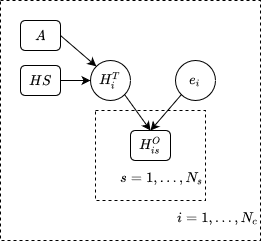
\includegraphics[width=\textwidth]{entropy_ME2.png}
		\caption{}
	\end{subfigure}
	\hfill
	\begin{subfigure}{0.5\textwidth}
		\centering
		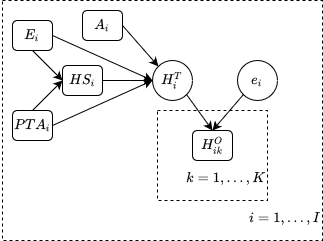
\includegraphics[width=\textwidth]{entropy_ME1.png}
		\caption{}
	\end{subfigure}
	%
	\caption[DAG for the measurement error model of entropy.]%
	{DAG for the measurement error model of entropy. (a) \textit{total effects} of hearing status, (b) \textit{direct effects} of hearing apparatus. Circles represent latent variables, squares observed values or covariates, and large discontinuous squares the nesting within specific units.}
	\label{fig:entropy_ME}
\end{figure}
%

First, figure \ref{fig:entropy_ME} depicts the DAG representation of the model. For the measurement error part, section \ref{ss_sect:outcome} reveals the (observed) entropy replicates $H^{O}_{ik}$ can represent multiple realizations of a child's \textit{true} entropy $H^{T}_{i}$, measured with error $e_i$. As a result, we can say the $k$'th entropy measure is nested within the $i$'th child, where $k=1, \dots, K$, $i=1, \dots, I$, $K = 10$ utterances, and $I = 32$ children.

Second, for the hypothesis part, we propose two sets of models. As we can see from Figure \ref{fig:entropy_ME}, the model in panel (a) use hearing status ($HS_{i}$) and hearing age ($A_{i}$) as covariates. The use of hearing status is justified as we are interested in comparing SI among groups, defined by the children's hearing characteristics (NH, HI/CI, and HI/HA). On the other hand, we expect hearing age\footnote{see section \ref{s_sect:children} to know how the variable is defined.} and its interaction with hearing status, to also have an effect on the \textit{true} SI measure, as previous evidence have shown the speech of HI children gradually approximate that of NH children \citep{Boonen_et_al_2019}.

Notice the model depicted in panel (a) is interested on (what we can call) \textit{total effects}, i.e. the effects of the hearing characteristics, not independent from the effects of the hearing apparatus (cochlear implant or hearing aid). This is important to understand for two reasons. Since a hearing apparatus is fitted onto a child depending on aspects such as the locus and severity of his(her) hearing impairment \citep{Korver_et_al_2017}: (1) such specific children's characteristics could confound the (beneficial) effects of using specific hearing apparatuses, while (2) because children are selected from a convenient sample, not representative of their respective populations (see section \ref{s_sect:children}), the need to control for such characteristics is paramount, if we seek to obtain effects that can generalize better and beyond our sample\footnote{follow the \textit{notes} folder, to see a graphical though experiment.}.

Considering the previous, we propose the model depicted in panel (b), where we control for the possible confounding variables etiology ($E_{i}$), \textcolor{blue}{as a proxy of locus}, and unaided PTA ($PTA_{i}$), as a proxy for hearing impairment severity. In that sense, the model would estimate (what we can call) the \textit{direct effects} of the hearing apparatus, independent of the children's characteristics.

Lastly, we proceed to use probabilistic programming to declare the algebraic structure of our models. Given the panel (a) model is nested within the panel (b) model, we declare only the model structure for the latter:
%
\begin{align}
	%
	\text{likelihood:} & \nonumber \\
	%
	H^{O}_{ik} & \sim \text{BetaProp} \left( H^{T}_{i}, M_{i} \right) \\ 
	%
	SI_{i} & \sim \text{N} \left( \mu_{i}, \sigma \right) \\
	%
	\nonumber \\
	%
	%
	\text{transformed parameters:} & \nonumber \\
	%
	H^{T}_{i} &= \text{logit}^{-1}( SI_{i} ) \\
	%
	M_{i} &= \kappa_{i} + 9 \\
	%
	\nonumber \\
	%
	%
	\text{linear predictor:} & \nonumber \\
	\mu_{i} & = \alpha_{HS[i]} + \beta_{HS[i]} (A_{i} - \bar{A}) + \alpha_{E[i]} + \beta_{P} PTA_{i} \\ 
	%
	\nonumber \\
	%
	%
	\text{priors:} & \nonumber \\
	%
	\sigma & \sim \text{Exp}(1) \\
	%
	\kappa_{i} & \sim \text{Exp}(2) \\
	%
	\alpha_{HS[i]} & \sim \text{N}(0, 0.5) \\
	%
	\beta_{HS[i]} & \sim \text{N}(0 , 0.3) \\
	%
	\alpha_{E[i]} & \sim \text{N}(0, 0.5) \\
	%
	\beta_{P} & \sim \text{N}(0, 0.3)
	%
\end{align}
%
\textcolor{blue}{where $\sigma_{H}$ denotes the variability of the replicated entropy measures, $\alpha_{HS[i]}$ and $\beta_{HS[i]}$ the intercept and slope of ``hearing age" per hearing status group, $\alpha_{E[i]}$ the intercept per etiology group, $\beta_{P}$ the slope for the PTA levels, and finally, $\text{logit}\left( H^{O}_{ik} \right) = \log \left[ H^{O}_{ik} / ( 1 - H^{O}_{ik} ) \right]$. Notice all the parameters are estimated in the logit scale and centered at $\bar{A}$, which denotes the minimum hearing age in the sample. Additionally, notice we have used mildly informative priors to state our uncertainty regarding the direction and magnitude of the effects\footnote{see \citet{Rivera_2021} (p. 18-19) for an intuition on prior elicitation.}. Finally, notice we can obtain the model in panel (a) if we do not consider etiology and PTA values in equation (2).}
%
%
%%%%%%%%%%%%%%%%%%%%%%%%%%%%%%%%%%%%
\subsubsection{Measurement models} \\
%
\textcolor{red}{(in process)}

\begin{comment}
	
	Identification of model:  
	soft identification (see \citet{Depaoli_2021}) 
	
	Considering the intelligibility of any stimulus is determined by three interrelated parties: the message, speaker, and listener, and that the inherent variability within each integrating part could be high, the current research assumes the utterances are equivalent among each other.
	
	It will consider the correlation with the entropy measure.
	%
	\begin{enumerate}
		\item \textbf{Dichotomous CJ (CJ-D):} the Bradley-Terry-Luce model (BTL) \citep{Bradley_et_al_1952, Luce_1959}, used when the comparative judgments are dichotomous (CJ-D), 
		%
		\item \textbf{Ordinal CJ (CJ-O):} the Generalized Bradley-Terry-Luce model BTL(k) \citep{Tutz_1986, Agresti_1992}, used when the comparative ordinal CJ (CJ-O).
		%
		\item \textbf{Absolute (holistic) judgments (HJ):}
	\end{enumerate}
\end{comment}
%
%
%%%%%%%%%%%%%%%%%%%%%%%%%%%%%%%%%%%%
\subsubsection{Integration models} \\
%
\textcolor{red}{(in process)} \\
%
%
%%%%%%%%%%%%%%%%%%%%%%%%%%%%%%%%%%%%%%%%%%%%%%%%%%%%%%%%%%%
\subsection{Model evaluation} \label{s_sect:evaluation}
%
As described in Section \ref{s_sect:models}, all seven models serve different but interrelated objectives.
%
%
%%%%%%%%%%%%%%%%%%%%%%%%%%%%%%%%%%%%
\subsubsection{Objective ranking}
%
As expected, model (1) allow us to construct the \textit{most objective} measure of a child's SI ranking. Moreover, using such model we will be able to test some research hypothesis of our interest.
%
%
%%%%%%%%%%%%%%%%%%%%%%%%%%%%%%%%%%%%
\subsubsection{Reliability}
%
The two remaining sets of models allow us to assess reliability in different ways. Under the second set of models (2a, 2b, 2c), we will be able to assess two forms of the inter-rater reliability: (a) the judges's reliability (JSR), and (b) the scale reliability, also known as the Scale Separation Reliability (SSR) \citep{Bramley_2015}. 

Following \citet{Fisher_1992} and \citet{Wright_1996} the measures were defined as follows:
%
\begin{align}
	JSR &= \frac{ G^{2}_{J} }{ (1 + G^{2}_{J}) }\; , \quad G_{J} = \frac{ \sigma_{\alpha} } { \sigma_{J} } \label{eq:JSR} \\
	%
	SSR &= \frac{ G^{2}_{\alpha} }{ (1 + G^{2}_{\alpha}) }\; , \quad G_{\alpha} = \frac{ \sigma_{\alpha} } { \sum_{i=1}^{C} se_{\alpha, i} } \label{eq:SSR}
\end{align}
%

\textcolor{red}{(in process)}

\begin{comment}
	compare the Scale Separation Reliability (SSR, an inter-rater reliability measure), coming from CJ methods, with others for other methods
	
	- No intra-rater reliability, also known as test-retest reliability (Verhavert_2018, Reliability_wiki_2022) 
	- No Inter-method reliability,  assesses the degree to which test scores are consistent when there is a variation in the methods or instruments used (Verhavert_2018, Reliability_wiki_2022) 
	- No comparison of SSR vs the true correlation of the latent scale and entropy measures 
	* Justification: (Verhavert_2018, p. 156) " simulation studies could resolve the inconclusiveness regarding the SSR as a correlation with the truth."
\end{comment}
%
%
%%%%%%%%%%%%%%%%%%%%%%%%%%%%%%%%%%%%
\subsubsection{validity}
%
the direction, magnitude, and quality of inference of the same research hypothesis outlined for Model (1), in the newly estimated models.

\textcolor{red}{(in process)}

\begin{comment}
	correlate latent scores (from different methods) with entropy measures (see research proposal)
	
	\textbf{critique:} What about decision statements or think at loud rating process? (is it possible), \citet{Lesterhuis_2018} has shown their usefulness, while \citet{Boonen_et_al_2020} signals the need to know about the inner working of judgment processes.
\end{comment}
%
%
%%%%%%%%%%%%%%%%%%%%%%%%%%%%%%%%%%%%
\subsubsection{time efficiency}
%
\textcolor{red}{(in process)}

\begin{comment}
	time needed for each judgement based on method from (Coertjens_et_al_2017).
	
	statistical efficiency has been researched on \citet{Leijon_et_al_2019} and \citet{Pritikin_2020} for the bayesian dichotomous BTL model and the ordinal BTL model, respectively.
\end{comment}
%
%
%%%%%%%%%%%%%%%%%%%%%%%%%%%%%%%%%%%%
\subsubsection{statistical efficiency}
%
\textcolor{red}{(in process)}